\documentclass{jfm}

% Compilation
\usepackage{silence} % Silence latex compiler warnings
\WarningFilter{latex}{Command \@xhline has changed} % Filter out warning
  % caused by redefinition between jfm.cls class and array (loaded by
  % siunitx)

% Import custom style file containing common packages and options
\setlength{\paperheight}{\pdfpageheight} % JFM class removes paperheight definition and hyperref raises a warning

% Import custom style file containing common packages and options
\usepackage{preamble}
\graphicspath{{./Figures/}}

% Discrete Fourier Transform
\newcommand{\GenP}{\hat{P}_m}
\newcommand{\POne}{\hat{P}_1}
\newcommand{\PTwo}{\hat{P}_2}
\newcommand{\PThree}{\hat{P}_3}
\newcommand{\PFour}{\hat{P}_4}

% Continuous Fourier Transform
\newcommand{\GenPk}{\hat{P}(\kappa)}
\newcommand{\PZerok}{\hat{P}(0)}

% Define custom math symbols
\DeclareMathOperator{\cn}{Cn}
\DeclareMathOperator{\sgn}{sgn}
\DeclareMathOperator{\Ur}{Ur}
\DeclareMathOperator{\Sk}{Sk}
\DeclareMathOperator{\As}{As}
%\DeclareMathOperator{\Bi}{Bi}

% Define \im as Roman i
\newcommand{\im}{\mathrm{i}}
% Replace epsilon with varepsilon
\renewcommand*{\epsilon}{\varepsilon}

%% Use \thalf and \squart commands from JFM class
%\newcommand\squart{\ensuremath{{\textstyle\frac{1}{4}}}}
%\newcommand\thalf{\ensuremath{{\textstyle\frac{1}{2}}}}

\linenumbers

\title{Wind-Induced Changes to Surface Gravity Wave Shape in Shallow Water}

\author{Thomas J. Zdyrski \and Falk Feddersen}

\begin{document}

\maketitle

\begin{abstract}
Wave shape (e.g.,\ wave skewness and asymmetry) impacts sediment
transport, beach morphology, and ship safety.
Previous work by the authors showed that wind (via changes in surface
pressure) affects wave shape in intermediate and deep water.
This effect was most pronounced as the depth ($kh$) decreased.
Here, this work investigates the interaction of wind and wave shape in
shallow water.
A multiple-scales analysis is applied to waves propagating over a
shallow ($kh \ll 1$), flat bottom with a variety of wind-induced
surface-pressure profiles, such as Jeffreys-type and generalized
Miles-type.
The shallow depth enhances the influence of wind on wave shape and
intensifies the waves' second-harmonic modes.
The results are compared to previous wave-tank experimental data and
numerical simulation results.
\end{abstract}

\section{Introduction}

\section{Problem Solving Technique}
We will treat the flow as irrotational and inviscid throughout the
fluid and neglect surface tension by restricting to wavelengths $\lambda
\gg \SI{2}{\centi\meter}$.
Furthermore, we restrict to planar wave propagation in the $+x$
direction and assume no mean Eulerian current $\overline{u} = 0$.
Finally, we choose a coordinate system with $z=0$ at the mean water level and
a horizontal, flat bottom located at $z=-h$.
Then, the governing equations are%
\footnote{
  We used the gauge freedom to absorb the Bernoulli ``constant'' $C(t)$
  in the dynamic boundary condition into the definition of $\phi$.
}
\begin{alignat}{2}
  0 &= \phi_{xx} + \phi_{yy} + \phi_{zz} &&\qq{on}
  -h < z < \eta \,, \label{eq:laplace}\\
  0 &= \phi_{z} &&\qq{on} z=-h \,, \label{eq:bottom_bc}\\
  \phi_{z} &= \eta_{t} + \phi_{x} \eta_{x} +
  \phi_{y} \eta_{y} &&\qq{on} z = \eta \,, \label{eq:kinematic_bc}\\
  \qq*{and} 0 &= \frac{p}{\rho_w} + g\eta + \phi_{t} +
  \frac{1}{2} \bqty{\phi_{x}^2 + \phi_{y}^2 + \phi_{z}^2} &&\qq{on} z=
  \eta \,. \label{eq:dynamic_bc}
\end{alignat}
We are seeking a spatially-periodic progressive wave:
\begin{gather}
  \eta(\vec{x},t) = \eta(x + \lambda, t) \,,
\end{gather}
with similar conditions on $\vec{u} \coloneqq \grad{\phi}$.
We are parameterizing our initial wave by four quantities: the depth,
bottom horizontal velocity, wave height, and wavelength.
We will choose a coordinate system where the bottom horizontal velocity
vanishes:
\begin{equation}
  \vec{u}\cross \vu{z} = 0 \label{eq:bot_bc_horz} \,.
\end{equation}
Additionally, we assume the surface pressure $p(x,t)$ is given by a
Jeffreys-type forcing \citep{jeffreys1925formation}:
\begin{equation}
  p(x,t) \propto \pdv{\eta(x,t)}{x} \,.
\end{equation}

\section{Normalization}
We will normalize by identifying characteristic scales.
The parameters we know \apriori are the wavenumber $k$, the (initial)
wave amplitude $a_0$, the depth $h$, the gravitational acceleration $g$,
and the wind speed $U$ expressed as a pressure magnitude $P \propto
\rho_a U^2$.
However, instead of using the conventional wavenumber $k \coloneqq 2 \pi
/ \lambda$, we will instead use an effective wavenumber $k_E \coloneqq 2
\pi/ L$ with $L$ a characteristic length over which $\eta$ changes
rapidly.
We want our analysis to apply to both periodic waves (for which
$\lambda$ is finite) and solitary waves (for which $\lambda$ is
infinite).
For reference, we will later find that $L \to \lambda$ for infinitesimal
waves, but $L$ corresponds to the full width at half maximum times $\pi/2$ for solitary
waves.
However, we will not make any such assumptions yet.

Denoting nondimensional variables with an accent, we have
\begin{equation*}
  \begin{aligned}
  x &= \frac{x'}{k_E} = h \frac{x'}{\sqrt{\mu}}\,, \\
  y &= \frac{y'}{k_E} = h \frac{y'}{\sqrt{\mu}}\,, \\
  z &= h z' \,,
  \end{aligned}
  \qquad
  \begin{aligned}
  t &= \frac{t'}{k_E\sqrt{g h}}
    = \frac{t'}{\sqrt{\mu}} \sqrt{\frac{h}{g}} \,, \\
  \eta &= a \eta' = h \epsilon \eta' \,, \\
  \phi &= \phi'\frac{a}{k_E}\sqrt{\frac{g}{h}}
    = \frac{\phi'\epsilon}{\sqrt{\mu}}\sqrt{g h^3} \,,
  \end{aligned}
  \qquad
  \begin{aligned}
  p &= \alpha p' \rho_w g a
    = \alpha \epsilon p' \rho_w g h \,, \\
  P &= \alpha P' \frac{\rho_w g}{k_E}
    = \frac{\alpha}{\sqrt{\mu}} P' \rho_w g h \,.
  \end{aligned}
\end{equation*}
Here, we have defined the parameters $\epsilon \coloneqq a_0/h$, $\mu
\coloneqq (kh)^2$, and $\alpha \coloneqq \order{P k_E/(\rho_w g
)}$.
Furthermore, we see that $\epsilon/\mu$ is (up to some numerical
prefactors) the Ursell number, $\Ur = H \lambda^2/d^3$.
Finally, note that $\order{p/\rho_w g h} = (\epsilon/\sqrt{\mu})
\order{P/\rho_w g h}$.

Using these definitions, our equations take the form
\begin{alignat}{2}
  0 &= \mu \pqty{\phi'_{x'x'} + \phi'_{y'y'}} + \phi'_{z'z'} &&\qq{on}
    -1 < z' < \epsilon \eta' \,, \label{eq:laplace_nondim} \\
  0 &= \phi'_{z'} &&\qq{on} z'=-1 \,, \label{eq:bottom_bc_nondim} \\
  \phi'_{z'} &= \mu \eta'_{t'} +
    \epsilon \mu \bqty{\phi'_{x'} \eta'_{x'} + \phi'_{y'} \eta'_{y'}}
    &&\qq{on} z' = \epsilon \eta' \,, \label{eq:kinematic_bc_nondim} \\
  0 &= \alpha p' +  \eta' + \phi'_{t'} + \frac{1}{2}
    \bqty{\epsilon \pqty{\phi_{x'}^{\prime \, 2} + \phi_{y'}^{\prime \,
    2}} +  \frac{\epsilon}{\mu} \phi_{z'}^{\prime \, 2}} &&\qq{on} z'=
    \epsilon \eta' \,.  \label{eq:dynamic_bc_nondim}
\end{alignat}
Note that this is equivalent to choosing a set of units wherein $h = g =
\rho_w = 1$.
The primes will be dropped henceforth for readability.

\section{Pressure Magnitude Estimation}
Now, we will estimate the wind speeds associated with different pressure
magnitudes $P$ over a simple sinusoidal wave.
For the deep water case, we related $P$ to the wind-induced energy growth
rate $\gamma$, which was then be related to the friction velocity $u_*$
through experimental measurements, which was finally converted to
$U_{10}$ wind speeds using logarithmic boundary layer theory.
Here, we encounter an issue: the experimental measurements are taken for
deep water, and are not necessarily expected to hold for shallow water
waves.

We will use the \citet{miles1957generation} theory for $P' \ll 1$ as a model%
\footnote{
  Though Miles does specialize to deep-water waves partway through the
  derivation, the equation we utilize is applicable to both shallow and
  deep water.
  The only difference is that $m = \rho_w/k$ and $s=\rho_a/\rho_w$,
  which Miles uses for deep water, should be replaced by
  $m=\rho_w\coth(kh)/k$ and $s = \tanh(kh) \rho_a/\rho_w$.
  Hence, the extra factor of $\tanh(kh)$ appearing in
  \cref{eq:miles_growth_rate}.
}%
, where
\begin{equation}
  p_M = k \rho_a U^2 \Re{(\tilde{\alpha} + \im \tilde{\beta}) \eta_a}
  \coloneqq k P_M \Re{ e^{\im \psi_P} \eta_a} \,.
\end{equation}
with $U$ a characteristic wind speed and $\eta_a$ the analytic
representation%
\footnote{
  The analytic representation of a real function $f(x)$ is $f(x) + \im
  \hat{f}(x)$ with $\hat{f}(x)$ the Hilbert transform of $f(x)$.
  For our purposes, only two representations will be relevant: the
  analytic representation of $\cos(x)$ is $e^{\im x}$ and that of
  $\sin(x)$ is $-\im e^{\im x}$.
}
of $\eta$.
This gives a relationship between the pressure magnitude $P$ and growth
rate $\gamma$ as
\begin{equation}
  \frac{\gamma}{\omega_0} \approx \frac{\gamma}{\Re{\omega}} \coloneqq
  \frac{1}{\omega E} \pdv{E}{t}
  = \tilde{\beta} \frac{\rho_a}{\rho_w} \frac{U^2}{c_0^2} \tanh(kh)
  = \tilde{\beta} \frac{\rho_a}{\rho_w} \frac{U^2 k}{g} \,,
  \label{eq:miles_growth_rate}
\end{equation}
with $c_0 = \sqrt{g\tanh(kh)/k}$ and $\omega_0 = c_0 k$.
Using our definition for $P_M \exp(\im \psi_P) = (\tilde{\alpha} + \im
\tilde{\beta}) \rho_a U^2$, we find
\begin{equation}
  \frac{\gamma}{\omega_0} \approx \frac{P_M k}{\rho_w g} \sin(\psi_P)
  = P'_M \alpha \sin(\psi_P)
  ,
\end{equation}
Note that this also matches the $P = \order{\epsilon}$ growth rate we
derive for the Jeffreys case (\ie $\psi_P = \pm \pi/2$) in
\cref{sec:energy_growth_rate}.

According to \citet{donelan2006wave}, the wind speed and growth rate
are related in shallow water by
\[
  \frac{\gamma}{\omega_0} = \frac{\rho_a}{\rho_w} (ak)
  \pqty{\frac{U_{\lambda/2}}{c_0} - 1}^2
  G \bqty{(ak)
  \pqty{\frac{U_{\lambda/2}}{c_0} - 1}^2}
\]
with $G[x] = b - q \mathcal{H}(x - 1)$ with $b = 4.91$, $q = 3.98$, and
$\mathcal{H}$ the Heaviside unit step function.
Finally, in the logarithmic boundary layer, we have
\[
  \frac{U_z}{\ln(z/z_0)} = \text{const}
  \implies U_{z} = U_{\lambda/2} \frac{\ln(z/z_0)}{\ln[\lambda/(2 z_0)]}
\]
with \citep{taylor2001dependence}
\[
  \frac{z_0}{H} = 1200 \pqty{\frac{H}{\lambda}}^{4.5}
\]
where $H$ is the wave height.
Combining this, we find
\[
  P'_M \alpha = \frac{\rho_a}{\rho_w} \csc(\psi_P)
  y \Bqty{b-qH[y - 1]}
\]
with
\[
  y \coloneqq
  \epsilon \sqrt{\mu}
  \pqty{\frac{U_{z}}{c_0} \frac{\ln(2400)+5.5\ln(\epsilon \sqrt{\mu}/\pi)}
    {\ln(1200) + 4.5 \ln(\epsilon \sqrt{\mu}/\pi) + \ln(H/z)} - 1}^2
\]
with $T$ the wave period.
If we take $\psi_P = 3\pi/4$ and $\rho_a/\rho_w = \num{1.225e3}$, we get
\[
  P'_M \alpha = \num{1.7e-3} y \Bqty{b-q \mathcal{H}[y - 1]}
\]
with $y$ given above.

If we take $\mu = \epsilon = 0.1$, $\rho_a/\rho_w = 10^{-3}$, $T =
\SI{10}{\second}$, $h = \SI{10}{\meter}$, and $z = \SI{10}{\meter}$, we
find
\[
  y = \num{3.2e-2} \pqty{U_{10} \SI{0.12}{\second\per\meter} - 1}^2
\]
For $U_{10} < \SI{56}{\meter\per\second}$, we have
\[
  P'_M \alpha = \SI{3.8e-6}{\second\squared\per\meter\squared} U_{10}^2
\]
For instance, $U_{10} = \SI{50}{\meter\per\second}$ gives
$P'_M \alpha = \num{6.5e-3} \approx \epsilon^2$.

If we instead consider laboratory conditions with $h=\SI{0.37}{\meter}$,
$kh = 1.2$, and $a_0/h = 0.14$ as in \citet{feddersen2005wind}, we
instead get
\[
  y = \num{0.17} \pqty{U_{10} \SI{0.73}{\second\per\meter} - 1}^2
\]
For $U_{10} > \SI{4.7}{\meter\per\second}$, we have
\[
  P'_M \alpha = \SI{1.5e-4}{\second\squared\per\meter\squared} U_{10}^2
\]
For instance, $U_{0.3} = \SI{8}{\meter\per\second}$ gives
$P'_M \alpha = \num{6.4e-3} \approx \epsilon^3$.

\section{Depth Dependence of \texorpdfstring{$\phi$}{Velocity Potential}}
First, we will determine the depth dependence of $\phi$ implied by
Laplace's equation.
We will do this be expanding $\phi$ in a Taylor series about the bottom
$z=-1$:
\begin{equation}
  \phi(x,y,z,t) = \sum_{n=0}^\infty (z+1)^n\phi_n(x,y,t) \,.
\end{equation}
Derivatives in the $\vu{z}$ direction give
\begin{equation}
  \pdv[2]{\phi}{z} = \sum_{n=2}^{\infty} (n-1)(n)(z+1)^{n-2}\phi_n =
  \sum_{n=0}^{\infty} (n+1)(n+2)(z+1)^n\phi_{n+2} \,.
\end{equation}
Denoting the horizontal gradient as $\grad_X \coloneqq
(\pdv{x},\pdv{y})$,
Laplace's equation, \cref{eq:laplace_nondim}, gives
\begin{equation}
  \mu \laplacian_X{\phi} + \pdv[2]{z} \phi = \sum_{n=0}^\infty
  (z+1)^n\pqty{\mu \laplacian_X \phi_n + (n+1)(n+2)\phi_{n+2}} = 0 \,.
\end{equation}
Since this holds for arbitrary $z \in [-1,\epsilon \eta]$, each
term in the series must vanish, giving a recursion relation:
\begin{equation}
  \phi_{n+2} = \frac{-\mu \laplacian_X{\phi_n}}{(n+1)(n+2)} \,.
\end{equation}

We assumed previously that we were dealing with a horizontal
bottom-boundary.
Then, our bottom-boundary condition, \cref{eq:bottom_bc_nondim}, implies
\begin{equation}
  \pdv{\phi}{z}\eval_{z=-1} = \pqty{\sum_{n=1}^\infty
  n(z+1)^{n-1}\phi_n}\eval_{z=-1} = \phi_1 = 0 \,.
\end{equation}
Therefore, the recursion relation shows that $\phi_n=0$ for all odd $n$.
Hence, we've found a partial expansion of $\phi$ in terms of $\mu$:
\begin{equation}
  \phi(x,y,z,t) = \sum_{n=0}^{\infty} (-\mu)^n \frac{(z+1)^{2n}}{(2n)!}
  \grad_{X}^{2n} \phi_0(x,y,t; \mu, \epsilon) \,.
  \label{eq:phi_expansion}
\end{equation}
If we assume $\mu \ll 1$, we have,
\begin{equation}
  \phi = \phi_0 - \frac{1}{2}\mu (z+1)^2\laplacian_X\phi_0 +
  \frac{\mu^2}{24}(z+1)^4\laplacian_X\laplacian_X\phi_0 +
  \order{\mu^3} \,.
\end{equation}

Using \cref{eq:laplace_nondim,eq:bottom_bc_nondim}, we have determined
the depth dependence of $\phi$.
Therefore, our remaining goal is to determine the form of $\eta$ and
$\phi_0$.
For convienence, we will define $\varphi \coloneqq \phi_0$, as we will
need to append more subscripts shortly.

Note that truncating our series $\phi_n$ at finite $n$ means
Laplace's equation is only satisfied approximately.
This is in contrast to the intermediate-depth water case, where we were
able to satisfy Laplace's equation identically at each order.

Substituting this series expansion into the two
remaining boundary equations,
\cref{eq:kinematic_bc_nondim,eq:dynamic_bc_nondim}, we have reduced our
system of equations to
\begin{gather}
  \eta_t + \grad_X{H}\vdot\pqty{\grad_X\varphi
    -\frac{1}{2}\mu H^2\laplacian_X\grad_X\varphi} =
    -H\laplacian_X\varphi
  +\frac{1}{6}\mu H^3\laplacian_X\laplacian_X\varphi +
    \order{\mu^2}, \\
  p + \eta + \varphi_{t} - \frac{1}{2}\mu H^2\laplacian_X\varphi_{t} +
    \frac{1}{2}\epsilon \pqty{\grad_X\varphi}^2 = \order{\mu^2}
    \,.
\end{gather}
Note that we have used the total depth $H\coloneqq 1+\epsilon\eta$.
These equations can be simplified slightly to give
\begin{gather}
  \eta_t + \grad_X(H\grad_X\varphi)
    -\frac{1}{6}\mu \grad_X\vdot(H^3\laplacian_X\grad_X\varphi) =
    \order{\mu^2} \,, \\
  p + \eta + \varphi_{t} - \frac{1}{2}\mu H^2\laplacian_X\varphi_{t} +
    \frac{1}{2}\epsilon\pqty{\grad_X\varphi}^2 = \order{\mu^2}
    \,.
\end{gather}

\subsection{Restrictions}
At this point, we will again restrict our attention to one-dimensional
waves:
\begin{gather}
  \eta_t + \pqty{H\varphi_x}_x
    -\frac{1}{6}\mu \pqty{H^3\varphi_{xxx}}_x =
    \order{\mu^2}, \label{eq:kinematic_bc_varphi} \,, \\
  \eta + \varphi_t - \frac{1}{2}\mu H^2\varphi_{txx} +
    \frac{1}{2}\epsilon\pqty{\varphi_x}^2 = \order{\mu^2} \,.
  \label{eq:dynamic_bc_varphi}
\end{gather}
Further, we will now assume $\order{\epsilon} = \order{\mu} \ll 1$ which
implies $\Ur = \order{1}$.

\section{Perturbation Expansion}
\label{sec:shallow_water}
We expand our timescale in terms of multiple timescales $t_n =
\epsilon^n t$ for $n= 0,1,2,\ldots$.
Thus, all time derivative become $\partial_t \to \partial_{t_0} +
\epsilon \partial_{t_1} + \ldots$.
Then, we expand our variables in an asymptotic series of $\mu$
\begin{align}
  \eta(x,t) &= \sum_{k=0}^{\infty} \epsilon^k
    \eta_{k+1}(x,t_0,t_1,\ldots) \,, \\
  \varphi(x,t) &= \sum_{k=0}^{\infty} \epsilon^k
    \varphi_{k+1}(x,t_0,t_1,\ldots) \,, \\
  p(x,t) &= \sum_{k=0}^{\infty} \epsilon^k p_{k+1}(x,t_0,t_1,\ldots)
    \,.
\end{align}

\section{\label{sec:intermediate} \texorpdfstring{Intermediate Wind:
$\alpha = \epsilon$}{Intermediate Wind}}
Here, we assume $\alpha \coloneqq P k/(\rho_w g) = \epsilon$.
\subsection{Zeroth Order Equations}
Collecting order-one terms $\order{\epsilon^0}$ from
\cref{eq:kinematic_bc_varphi,eq:dynamic_bc_varphi} gives
\begin{gather}
  \pdv{\eta_0}{t_0} + \pdv[2]{\varphi_0}{x} = 0 \,, \\
  \eta_0 + \pdv{\varphi_0}{t_0} = 0 \,.
\end{gather}
Eliminating $\eta_1$ from this gives
\begin{equation}
  \pqty{\pdv[2]{t_0} - \pdv[2]{x} } \varphi_0 = 0 \,.
  \label{eq:wave_eq}
\end{equation}
This is the standard one-dimensional wave equation.
This implies
\begin{equation}
  \varphi_0 = f_0(x-t_0,t_1) + g_0(x+t_0,t_1) \,.
  \label{eq:phi0_sol}
\end{equation}
Here, we have neglected the term linear in $t_0$ since we already set
our gauge condition $\varphi = f(t_0)$, and we neglected the term linear
in $x$ since we have chosen \cref{eq:bot_bc_horz} that $u =
\pdv*{\varphi}_x = 0$ at the bottom.
We will restrict to right-moving waves and take $g_0 = 0$.
This also gives
\begin{equation}
  \eta_0 = - \pdv{\varphi_0}{t_0} = f_0'(x-t_0,t_1) \,,
  \label{eq:eta0_sol}
\end{equation}
with $f_0'(x-t_0,t_1) \coloneqq \eval{\pdv*{\theta}
f_0(\theta,t_1)}_{\theta = x-t_0}$.

\subsection{\label{sec:int_first_order} First Order Equations}
Continuing to the next order of perturbation theory, we retain terms of
order $\order{\epsilon}$.
Inserting our previous solutions, \cref{eq:phi0_sol,eq:eta0_sol} yields
\begin{gather}
  \begin{aligned}
    \pdv{\eta_1}{t_0} + \pdv[2]{\varphi_{1}}{x} &=
      -\pdv{\eta_0}{t_1} - \pdv{x} \pqty{\eta_0 \pdv{\varphi_0}{x}} +
      \frac{1}{6} \frac{\mu}{\epsilon} \pdv[4]{\varphi_0}{x} \\
      &= -\pdv{f_0'}{t_1} - 2 f_0' f_0'' + \frac{1}{6}
      \frac{\mu}{\epsilon} f_0^{(4)} \,,
  \end{aligned}
  \\
  \begin{aligned}
    \eta_1 + \pdv{\varphi_1}{t_0} &= -p_0 -\pdv{\varphi_0}{t_1}
      + \frac{1}{2} \frac{\mu}{\epsilon} \frac{\partial^3 \varphi_0}
        {\partial t_0 \partial^2 x}
      - \frac{1}{2} \pqty{ \pdv{\varphi_0}{x} }^2 \\
    &= -\pdv{f_0}{t_1} - p_0 - \frac{1}{2} \frac{\mu}{\epsilon}
      f_0^{(3)} - \frac{1}{2} \pqty{f_0'}^2 \,,
  \end{aligned}
\end{gather}
with $f_0^{(n)} \coloneqq \eval{\pdv*[n]{\theta}
f_0(\theta,t_1)}_{\theta=x-t_0}$ the $n$-th derivative of $f_0$.

We can eliminate $\eta_1$ from these equations to give
\begin{equation}
  \pqty{\pdv[2]{x} - \pdv[2]{t_0}} \varphi_1 = -2 \pdv{f_0'}{t_1} +
    \pdv{p_0}{t_0} - 3 f_0' f_0'' - \frac{1}{3} \frac{\mu}{\epsilon}
    f_0^{(4)} \,.
\end{equation}
However, we assume all order $\varphi_{n}$ travel at the same speed; in
particular, this means we will choose
\begin{align}
  \varphi_1 = f_1(x-t_0,t_1,\ldots) \,, \label{eq:phi1_sol} \\
  \eta_1 = f_1'(x-t_0,t_1,\ldots) \,. \label{eq:eta1_sol}
\end{align}
Thus, the left hand side vanishes:
\begin{equation}
  \pdv{f_0'}{t_1} - \frac{1}{2} \pdv{p_0}{t_0} + \frac{3}{2} f_0' f_0''
    + \frac{1}{6} \frac{\mu}{\epsilon} f_0^{(4)} = 0\,.
\end{equation}
Converting back to $\eta_0$ gives
\begin{equation}
  \pdv{\eta_0}{t_1} - \frac{1}{2} \pdv{p_0}{t_0} + \frac{3}{2} \eta_0
  \eta_0' + \frac{1}{6} \frac{\mu}{\epsilon} \eta_0^{(3)} = 0\,.
\end{equation}

If we choose the Generalized Miles forcing type, then
\[
  p_0(x,t_0,t_1) = P_G \eta_0(x+\psi_P,t_0,t_1)
\]
This gives
\begin{equation}
  \pdv{\eta_0(x-t_0)}{t_1} + P_G \frac{1}{2} \eta_0'(x-t_0+\psi_P) +
  \frac{3}{2} \eta_0(x-t_0) \eta_0'(x-t_0) + \frac{1}{6}
  \frac{\mu}{\epsilon} \eta_0^{(3)}(x-t_0) = 0 \,.
  \label{eq:kdv_burgers_gen}
\end{equation}
This is the nonlocal Korteweg-de Vries (KdV) equation.
This is a rare, difficult-to-solve equation.

Alternatively, we now specialize to the Jeffreys forcing type,
\begin{equation}
  p_0 = P_J \pdv*{\eta_0}{x} = P_J f_0''
  \implies p'_0 = P'_J \sqrt{\frac{\mu}{\epsilon}} \pdv{\eta'_0}{x'}
  \,.
\end{equation}
This gives
\begin{equation}
   \pdv{f_0'}{t_1} + P_J \sqrt{\frac{\mu}{\epsilon}} \frac{1}{2} f_0'''
   + \frac{3}{2} f_0' f_0'' + \frac{1}{6} \frac{\mu}{\epsilon} f_0^{(4)}
   = 0 \,.
\end{equation}
Finally, we can replace $f_0' = \eta_0$ to yield
\begin{equation}
   \pdv{\eta_0}{t_1} + P_J \sqrt{\frac{\mu}{\epsilon}} \frac{1}{2}
   \eta_0'' + \frac{3}{2} \eta_0 \eta_0' + \frac{1}{6}
   \frac{\mu}{\epsilon} \eta_0^{(3)} = 0 \,.
  \label{eq:kdv_burgers}
\end{equation}
This is the Korteweg-de Vries (KdV)-Burgers equation, though the
``damping term'', $\eta_0''$ has a ``negative viscosity'' (which is
expected, since the wind should cause growth rather than decay).
The KdV-Burgers equation is not known to have any closed form solutions.

For the Jeffreys case, we get the KdV-Burgers equation.
We can solve this numerically, though we will need an initial condition.
We will choose the solutions of the ordinary KdV equation as our initial
condition: cnoidal or solitary waves (which are a special case of
cnoidal waves).

\section{Numerics}
In the general KdV case, we have
\begin{equation}
  \mathcal{A} \pdv{\eta_0}{t_1} + \mathcal{F} \pdv{\eta_0}{x} + \mathcal{B}
  \eta_0 \pdv{\eta_0}{x} + \mathcal{C} \pdv[3]{\eta_0}{x} = 0 \,.
\end{equation}
Using the solution in from \citet{dingemans1997water} (as quoted in
\citeauthor{brun2018convective}) and rescaling variables, the cnoidal
wave solution is
\begin{equation}
  \eta_0 = \eta_2 + H \cn^2\pqty{\frac{x-c_1 t}{\Delta} , m} \,,
\end{equation}
with
\begin{gather}
  \eta_2 = \frac{H}{m} \pqty{1 - m - \frac{E(m)}{K(m)}}
  \qq{and}
  \Delta = \sqrt{\frac{12 \mathcal{C}}{\mathcal{B}} \frac{m}{H}}
  \label{eq:nondim_cnoidal_params}
  \\
  \qq{and}
  c_1 = \frac{\mathcal{F}}{\mathcal{A}} + \frac{2}{3} \frac{H}{m}
  \frac{\mathcal{B}}{\mathcal{A}} \pqty{1 - \frac{1}{2} m - \frac{3}{2}
    \frac{E(m)}{K(m)}} \,.
\end{gather}
Note that the (nondimensional) wavelength $\lambda$ is
\begin{equation}
  \lambda = 2 K(m) \Delta = K(m) \sqrt{\frac{48
  \mathcal{C}}{\mathcal{B}} \frac{m}{H}} \,.
  \label{eq:nondim_lambda}
\end{equation}
Here, $\cn$ is one of the Jacobi elliptic functions, and $K(m)$ and
$E(m)$ are the complete elliptic integrals of the first and second kind,
respectively, with $m \in [0,1]$ the elliptic parameter.

The solitary wave solution is
\begin{equation}
  \eta_0 = H \sech^2\pqty{\frac{x - c_1 t_1}{\Delta}} \,,
\end{equation}
with
\begin{equation}
  \Delta = \sqrt{\frac{12 \mathcal{C}}{\mathcal{B}} \frac{1}{H}}
  \qq{and}
  c_1 = \frac{\mathcal{F}}{\mathcal{A}} + \frac{H \mathcal{B}}{3
    \mathcal{A}} \,.
\end{equation}
Note that the solitary wave is recovered from the cnoidal wave as $m \to
1$ (note $E(m)/K(m) \to 0$ as $m \to 1$), and the linear wave
approximation is recovered as $m \to 0$.
Here, $\abs{H}$ is an order-1 parameter and $\sgn(H) = \sgn(\mathcal{B}
\mathcal{C})$.
For our particular system, we have $\mathcal{A} = 1$, $\mathcal{B} =
3/2$, $\mathcal{C} = \mu/(6\epsilon)$, and $\mathcal{F} = 0$.

If we temporarily revert back to dimensional variables (with primes
denoting dimensionless), we have
\begin{equation}
  \begin{split}
  \frac{\eta_0}{\epsilon h} &= \eta_2' + H' \cn^2\pqty{\frac{k_E x - k_E
    \sqrt{gh} c_1' \epsilon t}{\Delta'}, m}
  \\
  \implies
  \eta_0 &= \epsilon h \eta_2' + \epsilon h H'
  \cn^2\pqty{\frac{k_E}{\Delta'} \bqty{x - \epsilon \sqrt{gh} c_1' t}, m}
  \\
  &\coloneqq \eta_2 + H \cn^2\pqty{\frac{x - c_1 t}{\Delta}, m} \,.
  \end{split}
\end{equation}
Here, we have defined the dimensional quantities $H$, $\eta_2$,
$\Delta$, and $c_1$:
\begin{gather}
  H = \epsilon h H'
  \qq{and}
  \eta_2 = \epsilon h \eta_2' = \frac{H}{m} \pqty{1 - m - \frac{E(m)}{K(m)}}
  \qq{and}
  \Delta = \frac{\Delta'}{k_E}
  \\
  \qq{and}
  c_1 = \epsilon \sqrt{gh} c_1' = \epsilon \sqrt{gh} \pqty{
    \frac{\mathcal{F}}{\mathcal{A}} + \frac{2}{3} \frac{H}{m}
    \frac{\mathcal{B}}{\mathcal{A}} \pqty{1 - \frac{1}{2} m - \frac{3}{2}
    \frac{E(m)}{K(m)}} }
\end{gather}
Given the conventional definition that $H = 2 a$, we have
\begin{equation}
  2 a = \epsilon h H' = a H' \implies H' = 2 \,.
\end{equation}
As $m \to 0$, we have $\cn \to \cos$, $K(m) \to \pi/2$ and $E(m) \to
\pi/2$, and we keep $H/m$ fixed.
This gives
\begin{equation}
  \eta_0 \to H \cos^2 \pqty{\frac{x-c_1 t}{\Delta}}^2
  = \frac{H}{2} \cos \pqty{\frac{2}{\Delta} \bqty{x-c_1 t}}
  \qq{as} m \to 0 \,.
\end{equation}
Since we want this to reduce to the usual $(H/2) \cos(k[x-c_1 t])$, we
define (for all $m$)
\begin{equation}
  k_E \coloneqq \frac{2}{\Delta}
\end{equation}
Note that \cref{eq:nondim_lambda} also means
\begin{equation}
  \lambda' = 2 K(m) \Delta' = 2 K(m) \Delta k_E = 4 K(m) \,.
\end{equation}
Note that, in particular, this means
\begin{equation}
  k = \frac{2 \pi}{\lambda} = \frac{2 \pi}{\lambda'} k_E
  = \frac{\pi}{2 K(m)} k_E \,.
\end{equation}
So, as $m \to 0$, $k \to k_E$, while $m \to 1$ yields $k \to 0$.

Finally, we can now fix $m$ as a function of $\mu$ and $\epsilon$:
\begin{equation}
  k_E = \frac{2}{\Delta} = \frac{2 k_E}{\Delta'}
  \implies \Delta' = 2 \,.
\end{equation}
However, using \cref{eq:nondim_cnoidal_params}, we have
\begin{equation}
  2 = \Delta ' = \sqrt{\frac{12 \mathcal{C}}{\mathcal{B}}
    \frac{m}{H'}}
  = \sqrt{\frac{12 \mathcal{C}}{\mathcal{B}} \frac{m}{2}}
  \implies m = \frac{2 \mathcal{B}}{3 \mathcal{C}} \,.
\end{equation}
For our particular values of $\mathcal{B} = 3/2$ and $\mathcal{C} =
\mu/(6 \epsilon)$, we have
\begin{equation}
  m = 6 \frac{\epsilon}{\mu} \,.
\end{equation}
Since $m \in [0,1]$, this implies $0 \le \epsilon \le \mu/6$.
Finally, note that since $m = 1$ gives the solitary wave solution, this
means that we have the requirement that
\begin{equation}
  \mu = 6 \epsilon
\end{equation}
for solitary waves; this is simply the well-known fact that the height
and width of a solitary wave satisfy a fixed relationship.

Therefore, the nondimensional equation we are solving is
\begin{equation}
  \mathcal{A} \pdv{\eta'_0}{t'_1} + \mathcal{F} \pdv{\eta'_0}{x'} + \mathcal{B}
  \eta'_0 \pdv{\eta'_0}{x'} + \mathcal{C} \pdv[3]{\eta'_0}{{x'}} = 0 \,.
\end{equation}
with $\mathcal{A} = 1$, $\mathcal{B} = 3/2$, $\mathcal{C} =
\mu/(6\epsilon)$, and $\mathcal{F} = 0$.
For our initial condition, we use
\begin{equation}
  \eta'_0(x) = \eta'_2 + 2 \cn^2\pqty{\frac{x'}{2} , m} \,,
\end{equation}
with
\begin{equation}
  \eta'_2 = \frac{2}{m} \pqty{1 - m - \frac{E(m)}{K(m)}}
\end{equation}

\section{Results}
Given the one free parameter $P k_E/(\rho_w g \epsilon)$ of the
KdV-Burgers equation \cref{eq:kdv_burgers} and the one-parameter family of
initial conditions indexed by the initial height $H_0$, we can now plot the
results for different $H_0$ and $P k_E/(\rho_w g \epsilon)$.
In particular, we are interested in different values of $\sgn(P)$:
recall that $P>0$ ($P<0$) implies wind in the same (opposite) direction
as the waves.

\begin{figure}
  \centering
  { % Put \phantomsubcaption in their own group to prevent it from
    % affecting the main figure's numbering
    \phantomsubcaption
    \label{fig:snapshots_solitary:a}
    \phantomsubcaption
    \label{fig:snapshots_solitary:b}
  }
  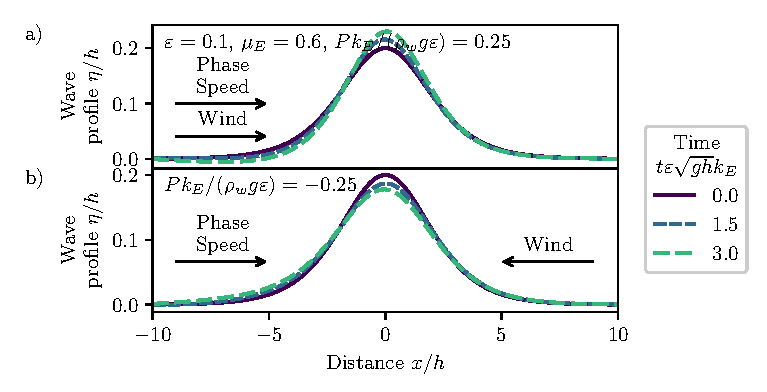
\includegraphics{Snapshots-Positive-Negative.eps}
  \caption{
    Evolution of a solitary wave profile under
    \subref{fig:snapshots_solitary:a}
    onshore and
    \subref{fig:snapshots_solitary:b}
    offshore Jeffreys forcing.
  }
  \label{fig:snapshots_solitary}
\end{figure}

In \cref{fig:snapshots_solitary}, we have plotted the wave profile
$\eta/h$ as a function of distance $x/h$ at different times $t \epsilon
\sqrt{g h} k_E$ and wind directions.
Both cases are plotted for initial wave steepness $\epsilon = 0.1$ and
pressure magnitude $\abs{P k_E/(\rho_w g \epsilon)} = 0.1$; the onshore
wind \subref{fig:snapshots_solitary:a} corresponds to $P>0$ while the
offshore wind \subref{fig:snapshots_solitary:b} has $P<0$.
We see that the initially symmetric solitary wave evolving over time
under the influence of \subref{fig:snapshots_solitary:a} onshore and
\subref{fig:snapshots_solitary:b} offshore winds.
For the onshore case \subref{fig:snapshots_solitary:a}, the wave grows,
steepens, and pitches forward, while the wave decays, becomes less
steep, and pitches backwards for the offshore case
\subref{fig:snapshots_solitary:b}.

\begin{figure}
  \centering
  { % Put \phantomsubcaption in their own group to prevent it from
    % affecting the main figure's numbering
    \phantomsubcaption
    \label{fig:xt_offset_solitary:a}
    \phantomsubcaption
    \label{fig:xt_offset_solitary:b}
  }
  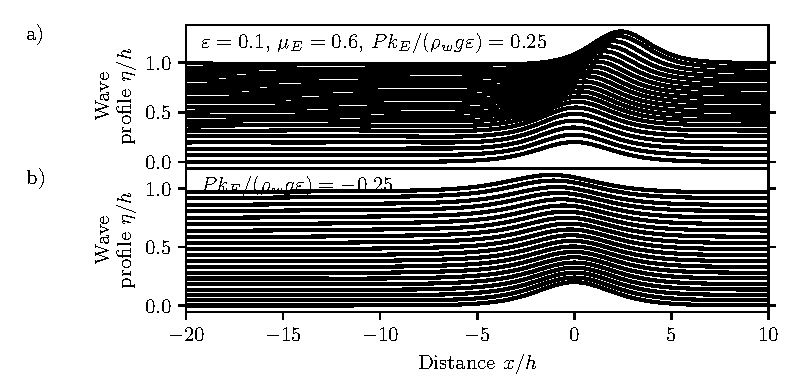
\includegraphics{XT-Offset.eps}
  \caption{
    An $x$-$t$ diagram of a solitary profile under
    \subref{fig:xt_offset_solitary:a}
    onshore and
    \subref{fig:xt_offset_solitary:b}
    offshore Jeffreys forcing.
    The lines are offset by $0.1 \eta/h$ per unit $t \epsilon \sqrt{g h}
    k_E$.
  }
  \label{fig:xt_offset_solitary}
\end{figure}

\Cref{fig:xt_offset_solitary} likewise shows the wave profile $\eta/h$
plotted against distance $x/h$ at different times $t \epsilon \sqrt{g h}
k_E$.
This time, each snapshot is shifted upwards, with a vertical
displacement of $0.1 \eta/h$ for each unit $t\epsilon \sqrt{g h} k_E$.
Again, both panels have an initial wave steepness of $\epsilon = 0.1$
and pressure magnitude $\abs{P k_E/(\rho_w g \epsilon)} = 0.1$, with
\subref{fig:xt_offset_solitary:a} corresponding to $P>0$ onshore wind,
and \subref{fig:xt_offset_solitary:b} corresponding to $P<0$ offshore
wind.
With both cases beginning from the exact same profile, it is clear to
see the steepening effect in \subref{fig:xt_offset_solitary:a} compared
to the decaying phenomenon in \subref{fig:xt_offset_solitary:b}.

\begin{figure}
  \centering
  { % Put \phantomsubcaption in their own group to prevent it from
    % affecting the main figure's numbering
    \phantomsubcaption
    \label{fig:statistics_solitary:a}
    \phantomsubcaption
    \label{fig:statistics_solitary:b}
    \phantomsubcaption
    \label{fig:statistics_solitary:c}
  }
  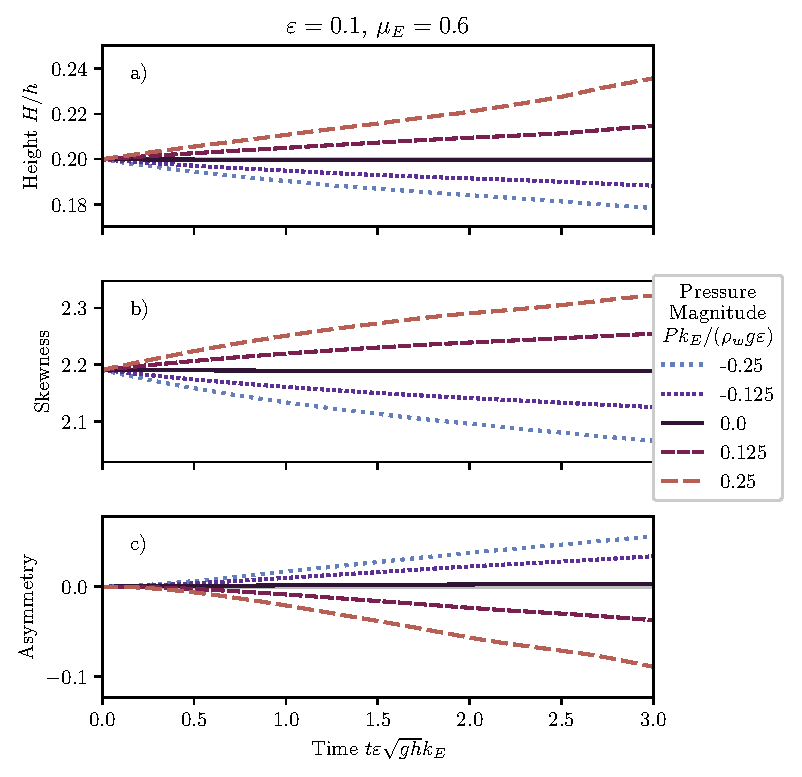
\includegraphics{Skew-Asymm-No-Peak.eps}
  \caption{
    Shape statistics of a solitary profile under onshore and offshore
    Jeffreys forcing.
    These include the
    \subref{fig:statistics_solitary:a}
    height,
    \subref{fig:statistics_solitary:b}
    skewness, and
    \subref{fig:statistics_solitary:c}
    asymmetry.
  }
  \label{fig:statistics_solitary}
\end{figure}

We have plotted various shape statistics for the solitary wave in
\cref{fig:statistics_solitary}.
The \subref{fig:statistics_solitary:a} wave height,
\subref{fig:statistics_solitary:b} skewness, and
\subref{fig:statistics_solitary:c} asymmetry all each plotted as
functions of time $t \epsilon \sqrt{g h} k_E$.
Additionally, each statistic is plotted for onshore wind ($P
k_E/(\rho_w g \epsilon) = 0.05$ and $0.1$), offshore wind ($P
k_E/(\rho_w g \epsilon) = -0.05$ and $-0.1$), and the unforced case
($P k_E/(\rho_w g \epsilon) = 0$).
All cases are plotted for initial steepness $\epsilon = 0.1$ for
$3/\epsilon = 30$ wave periods.
The height \subref{fig:statistics_solitary:a} begins at $H_0/h = 2
\epsilon = 0.2$ and shows the onshore wind
causing wave growth while the offshore wind causes decay, as was
observed in \cref{fig:snapshots_solitary,fig:xt_offset_solitary}.
The skewness of the initial profile is \num{2.19}, with onshore
(offshore) causing the wave to become more (less) skewed over time.
Finally, the initial profile has zero asymmetry, and the unforced case
$P=0$ maintains zero asymmetry over time.
However, the onshore wind causes the asymmetry to become negative
corresponding to a tilting backwards, while the offshore wind increases
the asymmetry causing the wave to tilt forwards.

\appendix

\section{Energy Growth Rate \label{sec:energy_growth_rate}}
As a useful check on our earlier estimation of the magnitude of $P'$, we
can derive the energy growth rate.
Multiplying \cref{eq:kdv_burgers} by $\eta_0$, we find
\begin{equation}
  \frac{1}{2} \pdv{t_1} \eta_0^2 + P_J \sqrt{\frac{\mu}{\epsilon}}
  \frac{1}{4} (\eta_0^2)'' - \frac{1}{2} P_J \sqrt{\frac{\mu}{\epsilon}}
  (\eta_0')^2 + \frac{1}{2} (\eta_0^3)' + \frac{1}{12}
  \frac{\mu}{\epsilon} (\eta_0^2)''' - \frac{1}{4} \frac{\mu}{\epsilon}
  \bqty{\pqty{\eta_0'}^2}' = 0 \,.
\end{equation}
Then, integrating over a wavelength gives
\begin{equation}
  \begin{split}
  &\pdv{t_1} \int_{-L/2}^{L/2} \frac{1}{2} \eta_0^2 \dd{x} \\
  &\qquad= \int_{-L/2}^{L/2} \frac{1}{2} P_J \sqrt{\frac{\mu}{\epsilon}}
    (\eta_0')^2 \dd{x} + \int_{-L/2}^{L/2} -P_J
    \sqrt{\frac{\mu}{\epsilon}} \frac{1}{4} (\eta_0^2)'' - \frac{1}{2}
    (\eta_0^3)' - \frac{1}{12} \frac{\mu}{\epsilon} (\eta_0^2)''' +
    \frac{1}{4} \frac{\mu}{\epsilon} \bqty{\pqty{\eta_0'}^2}' \dd{x}
  \\
  &\qquad=
  \int_{-L/2}^{L/2} \frac{1}{2} P_J \sqrt{\frac{\mu}{\epsilon}}
  (\eta_0')^2 \dd{x} + \eval{\bqty{-P_J \sqrt{\frac{\mu}{\epsilon}}
      \frac{1}{4} (\eta_0^2)'  - \frac{1}{2} (\eta_0^3) - \frac{1}{12}
      \frac{\mu}{\epsilon} (\eta_0^2)'' + \frac{1}{4}
      \frac{\mu}{\epsilon} \pqty{\eta_0'}^2}}_{-L/2}^{L/2}
  \\
  &\qquad=
  \int_{-L/2}^{L/2} \frac{1}{2} P_J \sqrt{\frac{\mu}{\epsilon}}
  (\eta_0')^2 \dd{x} \,.
  \end{split}
\end{equation}
Redimensionalizing, we find
\begin{equation}
  \frac{k}{\rho_w a^2} \frac{1}{\omega_0 \epsilon} \pdv{t} \int_{-L/2}^{L/2}
  \rho_w \eta^2 \dd{x} = \frac{1}{k a^2} \int_{-L/2}^{L/2} P_J'
  \sqrt{\frac{\mu}{\epsilon}} (\partial_x \eta)^2 \dd{x}
\end{equation}
or
\begin{equation}
  \frac{1}{\omega_0 E} \pdv{t} E =
  \epsilon
  \frac{
    \int_{-L/2}^{L/2} P_J' \sqrt{\frac{\mu}{\epsilon}} (\partial_x
    \eta)^2 \dd{x}
  }
  {
    \int_{-L/2}^{L/2} k^2 \eta^2 \dd{x}
  }
\end{equation}
with $E = \rho_w \int_{-L/2}^{L/2} \eta^2 \dd{x}$ the average
energy per wavelength.
The left-hand side is simply $\gamma/\omega_0$.
If, for simplicity, we consider a simple sinusoid $\eta_0 = A \cos(k x -
\omega_0 t)$, we find
\begin{equation}
  \frac{\gamma}{\omega_0} = \epsilon P_J' \sqrt{\frac{\mu}{\epsilon}} =
  \frac{P_J k}{\rho_w g} \sqrt{\frac{\mu}{\epsilon}} \,,
\end{equation}
where we used $\alpha = \epsilon$.

% Bibliography
\bibliographystyle{jfm}
\bibliography{references}

\end{document}
